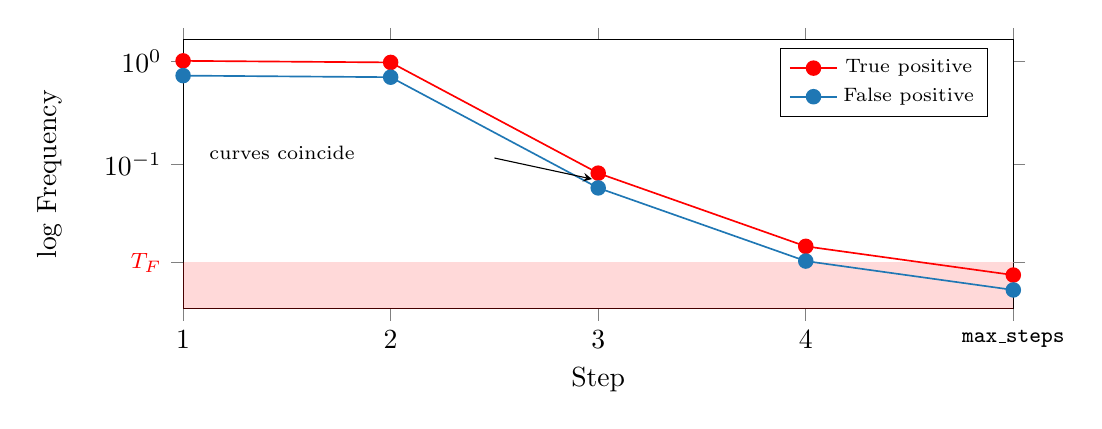
\begin{tikzpicture}
\begin{axis}[
log basis y={10},
width=\linewidth, height=5cm,
tick align=outside, tick pos=both,
xlabel={Step}, ylabel={$\log$ Frequency},
xmin=1, xmax=5, xtick={1,2,3,4,5},
xticklabels={1,2,3,4,\footnotesize\texttt{max\_steps}},
ymin=0.004, ymax=1.6, ymode=log,
ytick={1,0.1},
yticklabels={$10^{0}$,$10^{-1}$},
legend style={font=\scriptsize, at={(0.97,0.97)}, anchor=north east},
extra y ticks={0.0112},
extra y tick labels={\footnotesize $T_F$},
extra y tick style={yticklabel style={color=red}}
]
\path [draw=red, fill=red, opacity=0.15]
(axis cs:1,0.0112) --(axis cs:1,0.004) --(axis cs:5,0.004) --(axis cs:5,0.0112) --cycle;
% The two curves coincide; the false-positive curve is shifted down by a small
% constant factor so that both remain visible.
\addplot [semithick, red, mark=*, mark size=2.5] table {%
1 1
2 0.9656
3 0.0821
4 0.0161
5 0.0085
};
\addlegendentry{True positive}
\addplot [semithick, color={rgb,255:red,31;green,119;blue,180}, mark=*, mark size=2.5] table {%
1 0.72
2 0.6952
3 0.0591
4 0.0116
5 0.0061
};
\addlegendentry{False positive}
\node[font=\scriptsize, anchor=west] at (axis cs:1.08,0.13) {curves coincide};
\draw[->,>=stealth,thin] (axis cs:2.5,0.115) -- (axis cs:2.97,0.072);
\end{axis}
\end{tikzpicture}
